\section{Theory of Operations}

\subsection{Introduction}
The \textbf{I2C} module provides a complete implementation of the I2C (Inter-Integrated Circuit) protocol supporting both master and slave operation. It interfaces with the CPU via the APB bus and provides industry-standard I2C interface signals for connecting to external devices.

The module implements a flexible architecture with programmable clock rates, address recognition, and support for multiple operating modes including multi-master operation with arbitration detection.

\begin{figure}[h]
  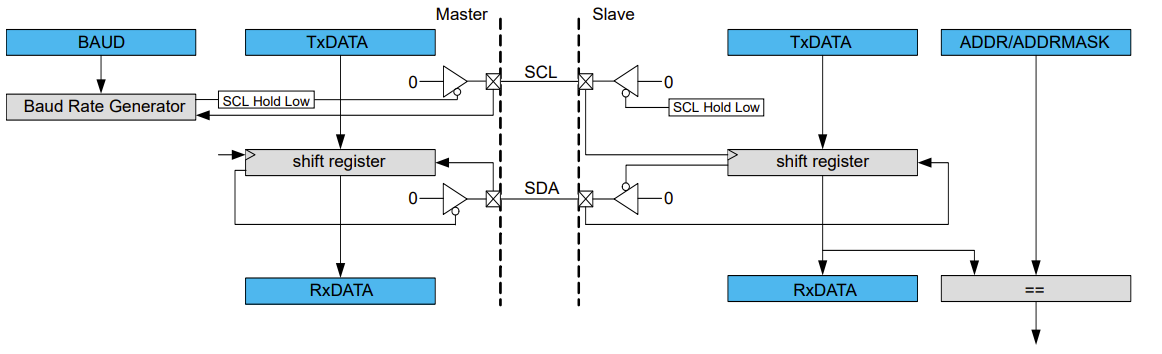
\includegraphics[width=0.90\textwidth]{images/i2c_block_diagram.png}
  \caption{I2C Block Diagram}\label{fig:block-diagram}
\end{figure}

The I2C module consists of several key components:
\begin{itemize}
    \item \textbf{APB Interface}: Handles register operations from the processor
    \item \textbf{Clock Generation}: Produces the SCL signal for master operation based on MBAUD value
    \item \textbf{State Machine}: Controls the I2C protocol sequence including START, data transfer, and STOP conditions
    \item \textbf{Shift Register}: Handles serial-to-parallel and parallel-to-serial conversion
    \item \textbf{Status Flags}: Provides feedback on operation completion and error conditions
\end{itemize}

When operating as a master, the module can initiate transactions by sending START conditions, transmitting addresses and data, receiving ACK/NACK responses, and terminating transactions with STOP conditions. In slave mode, it monitors the bus for its address, responds with ACK/NACK as appropriate, and transfers data according to the master's direction bit.

The module also supports advanced features like clock stretching (to allow more processing time) and multi-master arbitration for robust operation in complex systems.

\newpage
\subsection{Interface Timing}

The I2C module has a synchronous APB interface for register access and the standard I2C interface (SCL, SDA) for bus communication. The timing diagram shown below in Figure~\ref{fig:timing} represents a master write operation.

\begin{lstlisting}[language=Scala]
val myI2C = new I2C(
  p = BaseParams(
    dataWidth = 8,
    addrWidth = 16,
    regWidth = 8,
    clkFreq = 100
  ),
  formal = false
)
\end{lstlisting}

% \begin{figure}[h]
%   \includegraphics[width=\textwidth]{images/i2c_timing.png}
%   \caption{I2C Master Write Timing Diagram}\label{fig:timing}
% \end{figure}

This diagram illustrates a complete I2C master write transaction:

\begin{enumerate}
    \item \textbf{START Condition}: The master initiates a transaction by driving SDA low while SCL is high.
    \item \textbf{Address Phase}: The master transmits the 7-bit slave address followed by the R/W bit (0 for write).
    \item \textbf{Address ACK}: The slave acknowledges by pulling SDA low during the 9th clock cycle.
    \item \textbf{Data Write}: The master transmits 8 bits of data.
    \item \textbf{Data ACK}: The slave acknowledges the data byte.
    \item \textbf{STOP Condition}: The master terminates the transaction by releasing SDA from low to high while SCL is high.
\end{enumerate}

Throughout the transaction, the master controls the SCL clock line based on the MBAUD register setting. The status flags (WIF, RIF, RXACK) are updated to reflect the progress of the transaction.

When operating in slave mode, the module constantly monitors the bus for START conditions followed by its own address. Upon detection, it responds with ACK/NACK and transfers data according to the master's direction.

For operations requiring additional processing time, both master and slave can implement clock stretching by holding SCL low. This temporarily pauses the transaction until the stretching device is ready to continue.